% !TEX root=../../Thesis.tex
\chapter{Modeling Intersection Driving Scenarios}
\label{ch:modeling_intersection}

\begin{center}
  \textit{\textbf{RQ 1: How can RL be used to create a decision-making agent for autonomous driving through an unsignalized intersection?}}
  \end{center}
  \vspace{12pt}
  
To be able to derive algorithms for decision making we must first describe the mathematical formulation of the problem.  

\section{Intersection scenarios}
\tommy{show examples of intersections.}
\tommy{zone 0 - after intersection, zone 1 - conflict zone, zone 2 - right before the intersection, zone 3 - first obsereved interstion to zone 2}

\section{State space}
\tommy{Coordinate system, distances to intersection, position, velocity and accelration of other vehicles. abstract away the information about traffic lights, traffic signs, as intention}

\section{Action space}
\tommy{options, take way, give way, follow car}
short term goals presented in \paperLSTM.

\section{Transistion model}
\tommy{IDM, and other agents behaviors/intentions.}

\subsection{Simulation scenarios or simulator}
parameters, randomized cars. Behaviors. spawn rates and more. up to four cars. 

\section{Observation model}
\tommy{Everything in the state space except intention. Everything that is observable through the sensors in the car. }

\section{Reward function}
designing the reward model from the objective we are trying to achieve. this is not the optimal values. We are starting of a relative reward difference around 0 and 1. Then hand tune to get a performance close to the desired outcome. 

\section{Discussion}
Why is it hard. 
\tommy{zone 0 - after intersection, zone 1 - conflict zone, zone 2 - right before the intersection, zone 3 - first obsereved interstion to zone 2}

\begin{figure}[t]
	\mbox{\parbox{\textwidth}{
		\centering
		\begin{tikzpicture}
			\def\xstart{-7};

			\coordinate (p) at (3,0);
			\foreach \n/\w/\c in {z0/2/green,z1/2/red,z2/2.5/orange,z3/3.5/blue}{
				\node[rectangle,
				draw=none,
				anchor=east,
				text = black,
				fill = \c!60,
				minimum width = \w cm, 
				minimum height = 2cm] 
				(n) at (p) {\Huge \n};
				
				\coordinate (p) at (n.west);
			}

			% Crossing
			\draw[line width=0.5mm] (\xstart, 1) -- (-1, 1) -- (-1, 5);
			\draw[line width=0.5mm] (\xstart, -1) -- (-1, -1) -- (-1, -2);
			\draw[line width=0.5mm] (1, 5) -- (1, 1) -- (3, 1);
			\draw[line width=0.5mm] (1, -2) -- (1, -1) -- (3, -1);
			
			% cars
			\node[inner sep=0pt] (ego_car) at (-7,0)
			{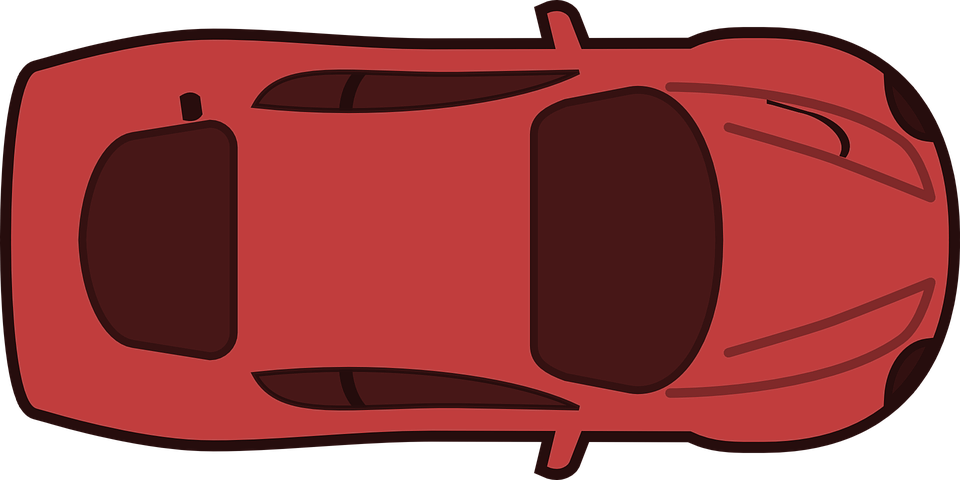
\includegraphics[width=.18\textwidth, angle=0]{figures/ego_car_top_down.png}};
			\node[inner sep=0pt] (target_car) at (0,4)
			{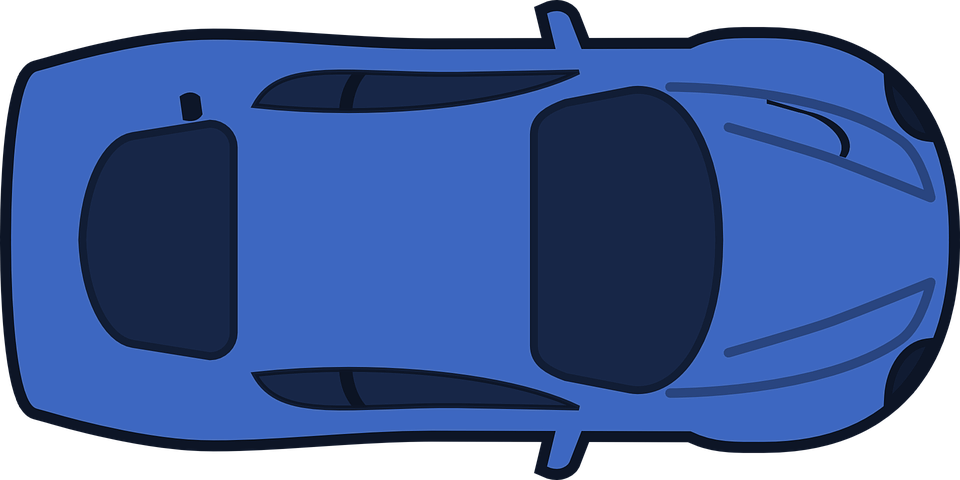
\includegraphics[width=.18\textwidth, angle=-90]{figures/target_car_top_down.png}};

	\end{tikzpicture}
	}}
	\caption{Intersection scenario divided into zones describing what is required of the decision maker in different zones}
	\label{fig:zones}
\end{figure}

With the \gls{mdp}, defined a typical intersection can be described as in Figure \ref{fig:zones}. From the figure we can divide the path of the ego vehicle into four zones. Starting from the end, zone 0 is the "safe zone" where the ego is our of danger and can return to nominal driving. Zone 1 is the conflict zone, this is where there is a possibility to collide with another vehicle. Zone 2 is critical decision zone, where this is the last chance the vehicle has to stop or cross. We define the size of this zone as the minimal distance the car needs to come to a complete stop to the start of the conflict zone. The final zone is zone 3, the information gathering zone, and is the furthest from the intersection and where the agent can observe the scenario and the other vehicles behavior over time. 

the goal is to reach zone 0, 
to do this the agent would want to minimize the time in zone 1, if there is chance of intersection with another car.
Because our actions are formulated as options and designed to be conformtable with lower acceleration rates. The size of zone 2 is dependent on the vehicels current speed, which is dependent on how the vehicle behaved in zone 3. 
Now there are two conflicting strategies, to minimize time in zone 1 the agent wants a high speed coming into the intersection. while it would want a low speed to shorten the zone 2 and the critical decision. 

If we know the intention of the other vehicles the stochasticity in zone 1 would be gone and the problem becomes a scheduling problem of creating a velocity profile that minimizes the time to cross.  

